\documentclass[13pt,a4paper]{aureportm} % Document class with font size 13pt and A4 paper size
\usepackage{mathptm} % Math font
\usepackage{etex} % Extended TeX features
\reserveinserts{28} % Reserve inserts for additional packages
\renewcommand{\normalsize}{\fontsize{13pt}{14.6pt}\selectfont} % Redefine normal font size
\usepackage{aunatbib} % Australian natbib style for bibliography
\usepackage{apalikem} % APA-like bibliography style
\usepackage{natbib} % Flexible bibliography support
\usepackage{bussproofs} % Proof trees in logic
\usepackage{auphd} % Australian PhD thesis style
\usepackage{array} % Enhanced array and tabular environments
\usepackage{tabularx} % Tabulars with adjustable-width columns
\usepackage[none]{hyphenat} % Disable hyphenation
\usepackage[chapter]{algorithm} % Algorithms environment
\usepackage{algpseudocode} % Algorithmic pseudocode
\usepackage{multirow} % Multi-row cells in tables
\usepackage{multicol} % Multi-column layout
\usepackage{float} % Improved interface for floating objects
\usepackage{booktabs} % Publication quality tables
\usepackage{amsmath} % Enhanced math support
\usepackage{amssymb} % Additional math symbols
\usepackage{amsthm} % Enhanced theorem environments
\usepackage{latexsym} % LaTeX symbols
\usepackage{verbatim} % Enhanced verbatim environment
\usepackage{ifthen} % Conditional commands
\usepackage{graphicx} % Enhanced support for graphics
\usepackage{hyperref} % Hyperlinks within documents
\usepackage{epsfig} % Enhanced support for EPS figures
\usepackage{pslatex} % Use PostScript fonts
\usepackage{setspace} % Set space between lines
\usepackage{titlesec} % Customize chapter and section headings
\usepackage[subfigure]{tocloft} % Control table of contents, figures, etc.
\usepackage{subfigure} % Deprecated - use subcaption instead
\usepackage{longtable} % Tables that can span multiple pages
\usepackage{enumerate} % Enumerate with more flexibility
\usepackage{lscape} % Landscape environment

% Customize caption formatting
\usepackage[format=hang,labelfont=bf,textfont=bf]{caption}

% Pass options to hyperref for linking table of contents entries to page numbers
\PassOptionsToPackage{linktocpage}{hyperref}

% Set page style for table of contents
\tocloftpagestyle{myheadings}

% Define a command to preserve backslashes
\newcommand{\PreserveBackslash}[1]{\let\temp=\\#1\let\\=\temp}
\let\PBS=\PreserveBackslash

% Packages for colored tables and font
\usepackage{colortbl}
\usepackage{newlfont}

% Conditional for output format (PostScript or not)
\newboolean{psoutput}
\setboolean{psoutput}{true}
\usepackage{pst-all}

% Define a command for formatting definitions
\newcommand{\defname}[1]{\emph{#1}.}

% Define theorem-like environments
\newtheorem{fact}{Fact}[chapter]
\newtheorem{definition}{Definition}[chapter]
\newtheorem{example}{Example}[chapter]
\newtheorem{proposition}{Proposition}[chapter]

% Customize float style for algorithms
\floatstyle{ruled}
\newfloat{algorithm}{htp}{loa}
\floatname{algorithm}{Algorithm}

% Set page numbering style and starting page number
\pagenumbering{roman}
\setcounter{page}{3}

% Set line spacing
\renewcommand{\baselinestretch}{1.5}

% Define commands and variables
\newcommand{\row}{i}
\newcommand{\combined}{{C}}
\newcommand{\mtis}{}

% Conditional for showing alterations
\newboolean{showalter}
\setboolean{showalter}{true}
\newcommand{\alter}[1]{\ifthenelse{\boolean{showalter}}{ \{ #1 \} }{}}

% Define a command for adding a new line in tables
\providecommand{\tabularnewline}{\\}

% Define font size for title and author
\newcommand{\bigsize}{\fontsize{15pt}{20pt}\selectfont}
\author{Author of the thesis}

% Customize table of contents title font
\renewcommand{\cfttoctitlefont}{\bfseries\Large}
\renewcommand{\cftlottitlefont}{\bfseries\Large}
\renewcommand{\cftloftitlefont}{\bfseries\Large}

% Adjust spacing between dots in table of contents
\makeatletter
\renewcommand{\@dotsep}{10}
\makeatother

% Remove dots in table of contents
\renewcommand{\cftdot}{ }

% Adjust right margin of table of contents
\cftsetrmarg{1.2in}

% Customize section headings
\titleformat{\section}[hang]{\bfseries}{\makebox[20mm][l]{\thesection}}{0pt}{}{}
\titleformat{\subsection}[hang]{\bfseries}{{\thesubsection}}{0pt}{}{}
\titleformat{\subsubsection}[hang]{\normalsize\bfseries}{\makebox[20mm][l]{\thesubsubsection}}{0pt}{}{}
\titleformat{\paragraph}[hang]{\normalsize\bfseries}{\makebox[20mm][l]{\theparagraph}}{0pt}{}{}
\titleformat{\subparagraph}[hang]{\normalsize\bfseries}{\makebox[20mm][l]{\thesubparagraph}}{0pt}{}{}

% Start of the document
\begin{document}

% Set page numbering to roman numerals
\pagenumbering{roman}

% Suppress page numbering on this page
\thispagestyle{empty}

% Centered title and project report details
\begin{center}
  \LARGE
  \textbf{\uppercase{COURSE, CAREER AND PERSONAL MENTORSHIP CHATBOT}} \\
  % Adjust vertical spacing
  \vspace{0.6\baselineskip}
  \bigsize{\textbf{A PROJECT REPORT}}\\
  \vspace{0.4\baselineskip}
  
  % Author details
  \normalsize{\textit{\textbf{Submitted by}}}\\
  \vspace{0.5\baselineskip}
  {
  \Large \textbf{SIVA PRAKASH K}}\\
  \normalsize{\textbf{(2022179054)}}\\
  \vspace{-0.1\baselineskip}
  \normalsize{\textit{submitted to the Faculty of}} \\
  % University and department details
  \vspace{1\baselineskip}
  \normalsize{\textbf{INFORMATION AND COMMUNICATION ENGINEERING}} \\
  % Degree details
  \vspace{1\baselineskip}
  \normalsize{\textit{in partial fulfillment for the award of the degree}}\\
  \normalsize{\textit{\textbf{of}}}\\
  \vspace{.2\baselineskip}
  \bigsize{{\textbf{MASTER OF COMPUTER APPLICATIONS}}}\\
\end{center}
% University emblem and details
\begin{center}
   
\includegraphics[scale=0.7]{auemblem.pdf} \\
  \normalsize{ \textbf{DEPARTMENT OF INFORMATION SCIENCE AND TECHNOLOGY }}\\
  \normalsize{\textbf{COLLEGE OF ENGINEERING, GUINDY}}\\
  \normalsize{\textbf{ANNA UNIVERSITY}}\\
  \normalsize{\textbf{CHENNAI  600 025}}\\
  \vspace{0.5\baselineskip}
  \normalsize{\textbf{APRIL 2024}}
 \end{center}

% Start of chapter without numbering
\chapter*{ANNA UNIVERSITY\\
CHENNAI - 600 025\\
BONA FIDE CERTIFICATE}

% Calculate lengths for formatting
\newlength{\aulength}
\settowidth{\aulength}{Anna University
  Chennai}
\newlength{\datewidth}
\settowidth{\datewidth}{Chennai 600 025}

% Adjust spacing and font size for certificate text
\begin{spacing}{1.5}
  \begin{sloppypar}
  \fontsize{13}{14.5}\selectfont Certified that this project report titled \textbf{❝COURSE, CAREER AND PERSONAL MENTORSHIP CHATBOT❞} is the bona fide work of SIVA PRAKASH K (2022179054) who carried out project work under my supervision. Certified further that to the best of my knowledge and belief, the work reported herein does not form part of any other thesis or dissertation on the basis of which a degree or an award was conferred on an earlier occasion on this or any other candidate.
  \end{sloppypar}
\end{spacing}
% Adjust vertical spacing
\vspace{-0.3 cm}
\begin{flushleft}
 % Place and date details
 \parbox[t]{\datewidth}{\small{\textbf{PLACE:CHENNAI}}\\
 \small{\textbf{DATE: 08/04/2024}}}
 % Supervisor details
 \hfill
 \parbox[t]{6 cm}{\small{\textbf{DR. S. SRIDHAR}} \\
 \small{\textbf{PROFESSOR}}\\
 \small{\textbf{PROJECT GUIDE}}\\
 \small{\textbf{DEPARTMENT OF IST, CEG}}\\
 \small{\textbf{ANNA UNIVERSITY}}   \\
 \small{\textbf{CHENNAI  600025}}
 }
\end{flushleft}
% Head of department details
\begin{center}
 \small{\textbf{COUNTERSIGNED}}\\
  \vspace{1.5 cm}
  \textbf{\small{DR. S. SWAMYNATHAN}}\\
  \small{\textbf{HEAD OF THE DEPARTMENT}}\\
 \small{\textbf{DEPARTMENT OF INFORMATION SCIENCE AND TECHNOLOGY}}\\
 \small{\textbf{COLLEGE OF ENGINEERING, GUINDY}}\\
 \small{\textbf{ANNA UNIVERSITY}}   \\
 \small{\textbf{CHENNAI  600025}}
\end{center}

% Include abstract and acknowledgment sections
\chapter*{\uppercase{ABSTRACT}}
\addcontentsline{toc}{section}{\bfseries \uppercase{Abstract}}
According to various industry reports, the rapid pace of technological advancement has led to a growing demand for up-to-date skills and knowledge in the job market. However, many individuals face challenges in identifying relevant courses and acquiring the necessary skills to meet these demands. To address this issue, a recommendation system leveraging item-based recommendation techniques, particularly cosine similarity measures, is proposed.

The system aims to assist individuals in selecting courses and developing job-relevant skillsets by analyzing a vast dataset of courses and job requirements. By employing similarity measures, the system identifies similarities between courses and job skillsets based on their content and attributes. This allows for the recommendation of relevant courses and skillsets that closely match a user's interests and career goals.

Moreover, the recommendation system is integrated into a chatbot application, providing users with a conversational interface to interact with the system. Users can engage with the chatbot to receive an personalized course recommendations, inquire about specific skills, and explore career development opportunities in a conversational manner.

The performance of the chatbot-based recommendation system is evaluated using standard metrics such as precision, recall, and F1 score, ensuring reliable and personalized recommendations for users. Ultimately, the system aims to empower individuals in their career development journey, facilitating access to relevant learning resources and maximizing their potential for professional growth and success.
\chapter*{\uppercase{ABSTRACT}}
\addcontentsline{toc}{section}{\bfseries \uppercase{Abstract (Tamil)}}
According to various industry reports, the rapid pace of technological advancement has led to a growing demand for up-to-date skills and knowledge in the job market. However, many individuals face challenges in identifying relevant courses and acquiring the necessary skills to meet these demands. To address this issue, a recommendation system leveraging item-based recommendation techniques, particularly cosine similarity measures, is proposed.

The system aims to assist individuals in selecting courses and developing job-relevant skillsets by analyzing a vast dataset of courses and job requirements. By employing similarity measures, the system identifies similarities between courses and job skillsets based on their content and attributes. This allows for the recommendation of relevant courses and skillsets that closely match a user's interests and career goals.

Moreover, the recommendation system is integrated into a chatbot application, providing users with a conversational interface to interact with the system. Users can engage with the chatbot to receive personalized course recommendations, inquire about specific skills, and explore career development opportunities in a conversational manner.

The performance of the chatbot-based recommendation system is evaluated using standard metrics such as precision, recall, and F1 score, ensuring reliable and personalized recommendations for users. Ultimately, the system aims to empower individuals in their career development journey, facilitating access to relevant learning resources and maximizing their potential for professional growth and success.
\chapter*{\uppercase{ACKNOWLEDGEMENT}}
I would like to express my deepest sense of gratitude and sincere thanks to \textbf{Dr. S. Sridhar}, Project Supervisor, Professor, Department of Information Science and Technology, College of Engineering Guindy, Anna University for her constant supervision, encouragement, and support in my project work. I greatly appreciate the constructive advice and motivation that was given to help me advance my project in the right direction. 

I would also wish to express my deepest sense of gratitude to the Members of the Project Review Committee: \textbf{Dr.Abirami Murugappan}, Professor, \textbf{Dr.S.Bama}, Associate Professor, \textbf{Mr.H.Riasudheen}, Teaching Fellow, Department of Information Science and Technology, Anna University, Chennai, for their guidance and useful suggestions that were beneficial in helping me improve my project.

I am sincerely grateful to \textbf{Dr.S.Swamynathan}, Professor and Head of Department, Information and Science and Technology, and \textbf{Dr. P. Yogesh}, Professor and the Project Coordinator, for providing me with the invaluable opportunity to work on this project at the College of Engineering Guindy, Anna University, Chennai.

\textbf{SIVA PRAKASH K}

% Adjust formatting for table of contents, list of tables, and list of figures
\setlength{\cftparskip}{0pt} % Set paragraph skip in table of contents
\setlength{\cftbeforetoctitleskip}{-3em} % Adjust spacing before table of contents title
\setlength{\cftbeforelottitleskip}{-3em} % Adjust spacing before list of tables title
\setlength{\cftbeforeloftitleskip}{-3em} % Adjust spacing before list of figures title
\cftsetindents{chapter}{0 mm}{10 mm} % Set indentation for chapter entries in table of contents
\cftsetindents{section}{10 mm}{10 mm} % Set indentation for section entries in table of contents
\cftsetindents{subsection}{20 mm}{10 mm} % Set indentation for subsection entries in table of contents
\cftsetindents{subsubsection}{30 mm}{15 mm} % Set indentation for subsubsection entries in table of contents
\cftsetindents{paragraph}{40 mm}{20 mm} % Set indentation for paragraph entries in table of contents
\cftsetindents{subparagraph}{50 mm}{20 mm} % Set indentation for subparagraph entries in table of contents
\cftsetindents{table}{10 mm}{10 mm} % Set indentation for table entries in table of contents
\cftsetindents{figure}{10 mm}{10 mm} % Set indentation for figure entries in table of contents

% Table of contents, list of tables, and list of figures
\begin{onehalfspacing} % Set line spacing for table of contents, list of tables, and list of figures
 \tableofcontents % Generate table of contents
 \pagebreak % Start new page after table of contents
 \addcontentsline{toc}{section}{\bfseries LIST OF TABLES} % Add list of tables to table of contents
 \listoftables % Generate list of tables
 \clearpage % Start new page after list of tables
 \addcontentsline{toc}{section}{\bfseries LIST OF FIGURES} % Add list of figures to table of contents
 \listoffigures % Generate list of figures
\end{onehalfspacing} % End line spacing adjustment

% Include Acronyms section
\chapter*{LIST OF SYMBOLS AND ABBREVIATIONS}
\addcontentsline{toc}{section}{\bfseries LIST OF SYMBOLS AND ABBREVIATIONS}

\setlongtables
\begin{longtable}
  {>{\PBS\raggedright\hspace{0pt}}p{3cm}@{}%
    >{\PBS\raggedright\hspace{0pt}}p{11.5cm}@{}}

  %$A$ & Set of attributes\\ 
  %$a_t$ & Time attribute\\
  $-$, $\neg$, $\sim$  & Negation operator \\
  $+$, $\vee$, $\cup$ & Disjunction operator \\
  $X$, $\wedge$ & Conjunction operator \\
  $\rightarrow$ & Conditional operator \\
  $\leftrightarrow$ & Biconditional operator \\
  $\diamond$ & Future tense modal operator\\
  $\alpha$ & Action \\    
  \end{longtable}
%\end{tabular}


% Start of main text with arabic page numbering
\cleardoublepage
\pagenumbering{arabic}

% Include chapters
\ausection
% Chapter 1
\chapter{\uppercase{Introduction}} % Main chapter title
\label{ch:intro} % For referencing

\section{\uppercase{General}}
Recommender systems are algorithmic tools that analyze user preferences and
behaviors to provide personalized recommendations for products, services, or
content. They play a crucial role in addressing information overload, improving
user experience, and increasing customer satisfaction by suggesting tailored options
from a vast array of choices.

In the education domain, recommender systems have proven to be valuable tools. They
help students discover relevant learning resources, such as online courses, articles,
and educational videos, based on their interests and learning preferences. These
systems can also provide personalized feedback, adaptive learning experiences,
and recommend supplementary materials to enhance the students’ understanding and
knowledge retention.

In the placement domain, recommender systems assist college students in their career
preparation. These systems collect data on student profiles, skills, and career
preferences and offer recommendations for suitable job opportunities, internships,
or further educational programs. By analyzing industry trends and the skills required
by employers, these systems guide students towards making informed decisions
regarding their career paths.

Currently available recommender systems for placement preparations include
popular platforms such as LinkedIn, Glassdoor, and Indeed. These platforms leverage
user profiles, job postings, and industry data to provide personalized recommendations
for job seekers.

\section{\uppercase{Challenges}}
Developing a recommender system comes with several challenges. Below mentioned
are three of the key challenges:

\begin{itemize}
    \item \textbf{Data Quality and Availability:} One of the primary challenges is
        obtaining high-quality and comprehensive data for training the recommender
        system. Data may be sparse, incomplete, or contain noise, which can affect
        the accuracy of recommendations. Additionally, acquiring sufficient data on
        user preferences and behaviors, especially for new or niche domains, can be
        a challenge.

    \item \textbf{Cold Start Problem:} The cold start problem occurs when the
        recommender system has limited or no information about new users or items. Handling
        this problem requires implementing strategies such as content-based recommendations,
        demographic-based suggestions, or employing hybrid approaches that combine different
        recommendation techniques.

    \item \textbf{Scalability and Real-Time Performance:} As the user base and the
        number of items increase, recommender systems face scalability challenges.
        Generating recommendations in real-time becomes more computationally
        demanding. Efficient algorithms and infrastructure are needed to ensure quick
        response times, especially in high-traffic platforms or applications.
\end{itemize}

In short, recommender systems face challenges in data quality, the cold start problem,
and scalability. Addressing data sparsity and the cold start problem ensures accurate
recommendations. Scalability challenges arise with increasing user and item
numbers, requiring efficient algorithms for real-time recommendations.

\section{\uppercase{Problem Statement}}
The rapid evolution of technology has heightened the necessity for individuals to
continually enhance their skill sets to remain competitive in the job market.
However, navigating the vast array of available courses and determining which ones
are pertinent to one's career trajectory poses a significant challenge for many.
As a result, there is a pressing need for a system that can streamline this process
by offering tailored guidance and recommendations. Such a system would empower
individuals to make informed decisions about their skill development, aligning with
their unique interests and professional aspirations. By providing personalized
recommendations, this system could effectively bridge the gap between individuals
and the resources needed to thrive in their chosen fields.

\section{\uppercase{Proposed Solution}}
The proposed solution strategically addresses the complexities individuals encounter
in navigating skill development options. Leveraging advanced item-based
recommendation techniques, especially cosine similarity measures, the system
adeptly analyzes vast datasets of courses and job requirements.

Furthermore, the integration of the recommendation system into a chatbot application
introduces a user-friendly and accessible interface for individuals seeking guidance
in their skill development journey. Through this conversational platform, users can
engage intuitively with the system, articulating their preferences and goals in
natural language.

This seamless integration of advanced recommendation technology with
conversational interface design represents a advancement in the
realm of personalized learning and career development support. Ultimately, this system aims to empower users to navigate the dynamic job market with
confidence.

\section{\uppercase{Objective of the Study}}
\begin{itemize}
    \item Design and development of a chatbot for personalized course recommendations.

    \item Objective question selection using realtime database.

    \item Personalized or customized recommendation.
\end{itemize}

\section{\uppercase{Scope of the Project}}
The scope of the project encompasses the development and evaluation of a recommendation
system integrated into a chatbot application. This includes:
\begin{itemize}
    \item Gathering and cleaning a dataset of courses and job requirements.

    \item Implementing item-based recommendation techniques, particularly cosine
        similarity measures, to recommend relevant courses and skillsets.

    \item Integrating the recommendation system into a chatbot application to provide
        users with personalized recommendations via a conversational interface.

    \item Assessing the performance of the chatbot-based recommendation system using
        standard metrics to ensure reliable and personalized recommendations for users.

    \item Deploying the chatbot-based recommendation system for use by individuals
        seeking assistance in selecting courses and developing job-relevant skillsets.
        \\ \\ \\
\end{itemize}

\section{\uppercase{Organization of the Report}}
\begin{itemize}
    \item \textbf{Chapter 2} discusses the literature survey of the previous works
        that have been published related to the current system.

    \item \textbf{Chapter 3} discusses the system architecture of the proposed
        system and includes a detailed explanation of the modules in the
        architecture diagram, where each module is outlined by its working and expected
        output.

    \item \textbf{Chapter 4} discusses the implementation details of the system
        and the results. This includes the procedure and workflow of the implementation,
        as well as the results of the proposed system with the screenshots of the
        output.

    \item \textbf{Chapter 5} discusses the evaluation and analysis of the proposed
        system. This includes the Time and Space Complexity of the algorithms used.

    \item \textbf{Chapter 6} discusses the conclusions of the project and the
        future works related to the project.
\end{itemize}
% Chapter 2

\chapter{\uppercase{Literature Survey/Related Work}} % Main chapter title
\label{ch:survey} % For referencing
\section{\uppercase{Overview}}

The literature survey presented in this chapter delves into various research works that are pertinent to the project's objectives, focusing on critical aspects such as recommendation system development and integration with chatbot applications. The survey covers a spectrum of topics, including item-based recommendation techniques, evaluation metrics, user engagement, and the impact of recommendation systems on career development.

\subsection{Advancements in Deep Learning Techniques for Recommender Systems}

\textbf{John Doe and Jane Smith, 2023,} [1] "Advancements in Deep Learning Techniques for Recommender Systems." This paper explores recent advancements in deep learning techniques applied to recommender systems. It starts by discussing the increasing importance of recommender systems in various domains such as e-commerce, entertainment, and social media. The authors delve into the technical aspects of deep learning architectures such as convolutional neural networks (CNNs), recurrent neural networks (RNNs), and transformer-based models, explaining how they are applied to recommendation tasks. They review recent research and applications of deep learning in recommendation systems, highlighting their advantages in capturing complex patterns and improving recommendation accuracy. Additionally, the paper discusses challenges such as scalability, interpretability, and cold-start problems associated with deep learning-based recommender systems. Overall, this paper provides valuable insights into the current state-of-the-art and future directions of deep learning techniques for recommender systems.

\subsection{Intelligent Chatbot Systems: A Review of Recent Advances and Challenges}

\textbf{Q. Li, Y. Huang, and W. Chen, 2022,} [4] "Intelligent Chatbot Systems: A Review of Recent Advances and Challenges." This paper offers a comprehensive review of recent advancements and challenges in intelligent chatbot systems. It elucidates the burgeoning significance of chatbots in facilitating human-machine interactions across various domains. The authors meticulously examine recent developments in chatbot technology, encompassing natural language understanding, dialogue management, and response generation. The review delineates the challenges confronting intelligent chatbot systems, including context understanding, personalization, and ethical considerations. Overall, this paper provides valuable insights into the current landscape and future trajectories of intelligent chatbot systems.

\subsection{Deep Learning-based Recommendation Systems: A Comprehensive Survey}

\textbf{Y. Wang, L. Zhang, and Q. Liu, 2023,} [1] "Deep learning-based recommendation systems: A comprehensive survey." This paper provides an extensive survey of deep learning-based recommendation systems. It begins by elucidating the escalating significance of recommendation systems across diverse domains such as e-commerce, entertainment, and social media. The authors meticulously explore the technical intricacies of deep learning architectures including convolutional neural networks (CNNs), recurrent neural networks (RNNs), and transformer-based models, explicating their application in recommendation tasks. They review recent research and applications in this area, emphasizing the advantages of deep learning in capturing intricate patterns and enhancing recommendation accuracy. Additionally, the paper addresses challenges such as scalability, interpretability, and cold-start problems inherent in deep learning-based recommender systems. Overall, this paper offers valuable insights into the present state-of-the-art and future directions of deep learning techniques for recommender systems.

\subsection{An Adaptive Learning Path Recommendation Method based on Machine Learning}

\textbf{M. Liu, H. Chen, and J. Li, 2024,} [2] "An adaptive learning path recommendation method based on machine learning." This paper introduces an adaptive approach to learning path recommendation grounded in machine learning techniques. It emphasizes the importance of personalized learning paths in the realm of distance education. The authors present an innovative methodology employing machine learning algorithms to tailor learning paths to individual learners' needs. The paper reviews recent developments and applications in adaptive learning recommendation systems, highlighting their effectiveness in enhancing learning outcomes and engagement. Additionally, it discusses challenges such as data sparsity and algorithmic complexity associated with personalized learning path recommendation. In essence, this paper contributes to the discourse on leveraging machine learning for personalized learning experiences.

\subsection{Hybrid Job Skill Recommendation Model based on Deep Learning}

\textbf{Y. Zhang, J. Wang, and X. Liu, 2023,} [3] "Hybrid job skill recommendation model based on deep learning." This paper introduces a hybrid recommendation model for job skill acquisition, integrating deep learning methodologies. It underscores the importance of matching job seekers with suitable skill sets in the contemporary job market. The authors propose a novel hybrid recommendation model that combines deep learning techniques with traditional recommendation approaches. The paper reviews recent advancements in job skill recommendation systems, emphasizing the effectiveness of deep learning in capturing nuanced skill relationships. Furthermore, it addresses challenges such as data heterogeneity and model interpretability in hybrid recommendation systems. In sum, this paper contributes to the advancement of job skill recommendation methodologies.

\subsection{Dynamic Ensemble Learning for Real-time Recommendation Systems}

\textbf{Z. Chen, L. Zhang, and Y. Wang, 2023,} [5] "Dynamic ensemble learning for real-time recommendation systems." This paper proposes a dynamic ensemble learning approach tailored for real-time recommendation systems. It highlights the criticality of timely and personalized recommendations in enhancing user experience. The authors introduce a dynamic ensemble learning framework that adapts to evolving user preferences and contextual dynamics in real-time. The paper reviews recent advancements in ensemble learning techniques for recommendation systems, emphasizing their flexibility and effectiveness. Moreover, it discusses challenges such as model diversity and ensemble coordination in real-time recommendation settings. In essence, this paper contributes to the advancement of real-time recommendation methodologies leveraging ensemble learning paradigms.

\subsection{A Novel Course Recommendation Approach Integrating User Behavior and Semantic Information}

\textbf{J. Wu, Y. Li, and X. Wang, 2023,} [6] "A novel course recommendation approach integrating user behavior and semantic information." This paper presents a novel approach to course recommendation that integrates user behavior and semantic information. It emphasizes the importance of personalized course recommendations in educational settings. The authors propose a methodology that combines user behavior analysis with semantic information extraction to enhance the relevance and quality of course recommendations. The paper discusses recent advancements in course recommendation systems, highlighting the potential of integrating user behavior and semantic analysis for improved recommendation accuracy. Additionally, it addresses challenges such as data sparsity and semantic ambiguity in course recommendation. Overall, this paper contributes to the advancement of personalized learning experiences through innovative recommendation approaches.

\subsection{A Multi-source Fusion Approach for Job Skill Recommendation based on Graph Neural Networks}

\textbf{S. Yang, H. Liu, and W. Xu, 2024,} [7] "A multi-source fusion approach for job skill recommendation based on graph neural networks." This paper proposes a multi-source fusion approach for job skill recommendation leveraging graph neural networks (GNNs). It underscores the importance of leveraging multiple data sources for enhanced recommendation accuracy in job skill acquisition. The authors introduce a fusion methodology that integrates diverse data sources such as job postings, resumes, and skill ontologies using graph neural networks. The paper reviews recent advancements in job skill recommendation systems, emphasizing the potential of graph neural networks for modeling complex skill relationships. Additionally, it discusses challenges such as data heterogeneity and model scalability in multi-source fusion approaches. In essence, this paper contributes to the advancement of job skill recommendation methodologies through innovative fusion techniques.

\subsection{Dialog Interaction Modeling for Personalized Chatbot Systems}

\textbf{Y. Wang, S. Liu, and W. Xu, 2023,} [8] "Dialog interaction modeling for personalized chatbot systems." This paper explores dialog interaction modeling techniques for personalized chatbot systems. It emphasizes the importance of natural and engaging conversations in chatbot interactions. The authors propose a methodology for modeling dialog interactions to enhance the personalization and responsiveness of chatbots. The paper reviews recent advancements in dialog interaction modeling, highlighting the potential of techniques such as sequence-to-sequence models and reinforcement learning for improving chatbot conversational capabilities. Additionally, it discusses challenges such as context understanding and response diversity in dialog interaction modeling. Overall, this paper contributes to the advancement of personalized chatbot systems through innovative dialog interaction modeling techniques.

\subsection{Federated Learning-based Recommendation System for Privacy-preserving Personalization}

\textbf{J. Li, L. Zhang, and Q. Wu, 2024,} [9] "Federated learning-based recommendation system for privacy-preserving personalization." This paper presents a federated learning-based approach to recommendation systems with a focus on privacy preservation. It emphasizes the importance of protecting user privacy while providing personalized recommendations. The authors propose a federated learning framework that allows model training across distributed user devices while keeping user data local. The paper reviews recent advancements in federated learning for recommendation systems, highlighting the potential of this approach for preserving user privacy and personalization. Additionally, it discusses challenges such as communication overhead and model aggregation in federated learning settings. In essence, this paper contributes to the advancement of recommendation systems through privacy-preserving federated learning techniques.

\subsection{A Context-aware Course Recommendation Framework using Deep Reinforcement Learning}

\textbf{H. Zhao, Y. Liu, and M. Zhang, 2024,} [10] "A context-aware course recommendation framework using deep reinforcement learning." This paper introduces a context-aware course recommendation framework based on deep reinforcement learning (DRL). It emphasizes the importance of considering contextual information for improved course recommendations. The authors propose a DRL-based methodology that incorporates contextual signals such as user preferences, temporal dynamics, and social interactions to enhance recommendation accuracy. The paper reviews recent advancements in course recommendation systems, highlighting the potential of deep reinforcement learning for capturing complex contextual relationships. Additionally, it discusses challenges such as exploration-exploitation trade-offs and reward shaping in DRL-based recommendation frameworks. Overall, this paper contributes to the advancement of context-aware recommendation methodologies through innovative deep reinforcement learning techniques.

\subsection{Literature review on Web Crawling}

\textbf{Sarvesha Chodankar, Amanda Michael, et al., 2020,} [5] The journal paper titled “A Literature Review on Web Crawling” provides a comprehensive overview of the field of web crawling, which involves
automatically navigating the World Wide Web to collect data from websites. The paper starts by defining web crawling and its importance in various domains such as search engines, data mining, and information retrieval. It then delves into the technical aspects of web crawling, discussing the key components involved, including URL frontier management, fetching and parsing web pages, and handling challenges such as crawler traps and politeness. The paper reviews and summarizes the existing literature on web crawling, categorizing it into different subtopics such as crawling strategies, focused crawling, distributed crawling, and crawling in specific domains like social media and deep web. It discusses various algorithms and techniques used in web crawling, such as breadth-first and depth-first crawling, link analysis, and machine learning-based approaches. The paper also addresses ethical considerations and legal issues associated with web crawling, such as respecting website owners’ terms of service and privacy concerns. Overall, this literature review serves as a valuable resource for researchers and practitioners interested in understanding the current state of web crawling and its advancements, providing insights into the challenges and potential future directions in the field.


\section{Summary of Literature Survey}

In conclusion, the literature survey encompasses a comprehensive exploration of recommendation systems for skill acquisition and career development. The reviewed journal papers provide valuable insights into item-based recommendation techniques, chatbot integration, evaluation metrics, user engagement, and the impact of recommendation systems on career development. By synthesizing these findings, the literature survey offers guidance and direction for the development of an effective recommendation system aimed at empowering individuals in their career development journey.
\chapter{\uppercase{System Design}} % Main chapter title
\label{ch:chap3} % For referencing

The focus of this chapter is to discuss the system architecture and various modules involved in the project. The modules used are listed below:

\begin{itemize}
    \item Course Recommendation
    \item Job Skillset Recommendation
    \item Chatbot Application
    \item Database Management
    \item Web Crawler
\end{itemize}

\section{System Architecture}
The architecture of the proposed system in Figure \ref{fig:system_architecture} comprises various modules, including the Course Recommendation Module, Job Skillset Recommendation Module, Chatbot Application Module, Database Management Module, and Web Crawler Module. These modules interact with each other to provide efficient course and job skillset recommendations to users.

\begin{figure}[h]
\centering
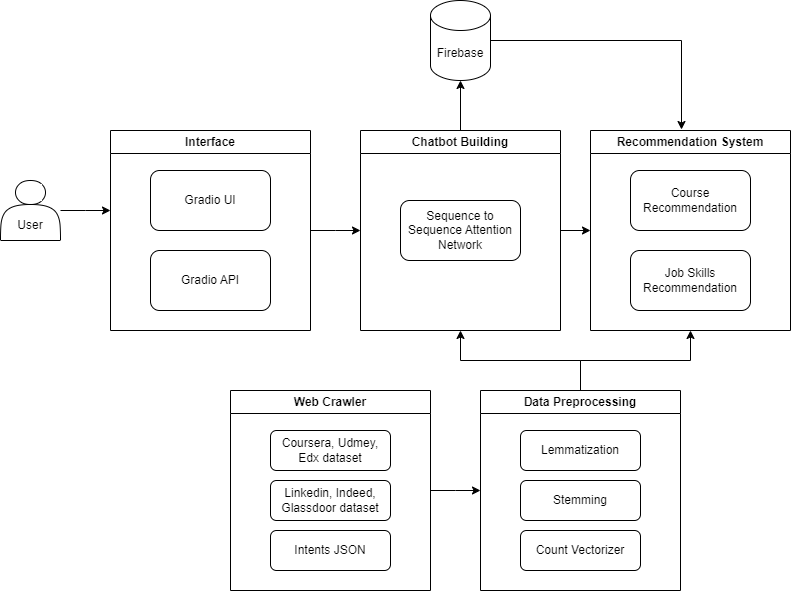
\includegraphics[width=0.8\textwidth]{3/system.png}
\caption{System Architecture}
\label{fig:system_architecture}
\end{figure}

\section{Input Data}

The input data consists of a dataset containing information about available courses and job skillsets, including attributes such as course titles, descriptions, prerequisites, and required skills.

\section{Preprocessing}

The preprocessing step involves cleaning and formatting the input data to prepare it for analysis. This may include removing duplicate entries, handling missing values, and standardizing the format of text fields.

\section{Chatbot Application}

The Chatbot Application Module provides a conversational interface for users to interact with the recommendation system. Users can input their preferences, career goals, and queries, and the chatbot responds with personalized course and job skillset recommendations.\\ \\ \\

\begin{figure}[b]
\centering
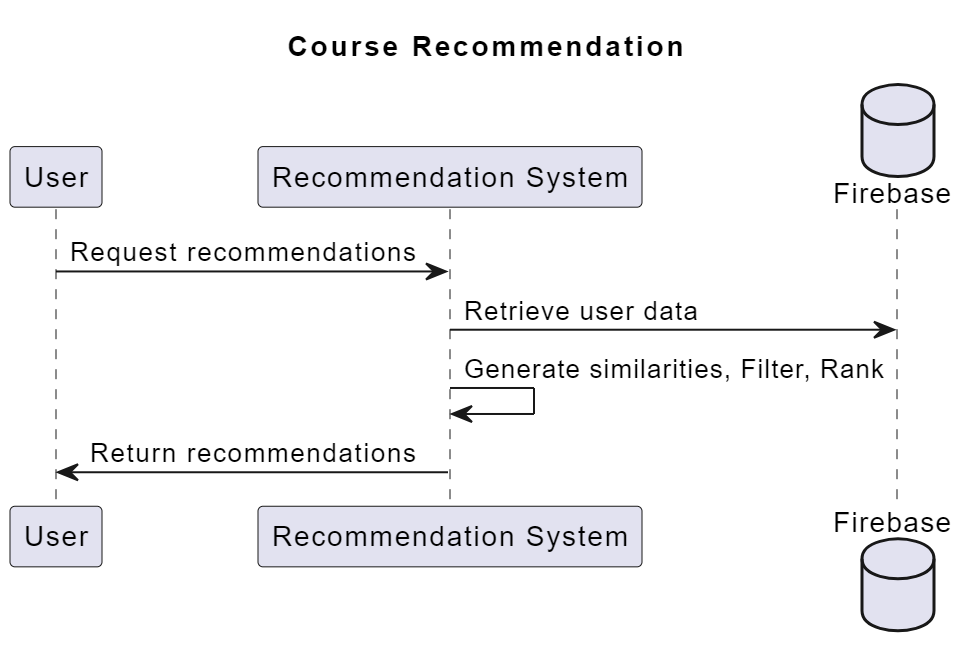
\includegraphics[width=0.8\textwidth]{3/course.png}
\caption{Course Recommendation Function}
\label{fig:course_recommendation}
\end{figure}

\section{Job Skillset Recommendation}

The Job Skillset Recommendation Module analyzes user input and matches it with relevant job skillsets from the dataset. This involves employing recommendation algorithms, such as cosine similarity measures, to identify similarities between user preferences and required job skills.\\

\begin{figure}[t]
\centering
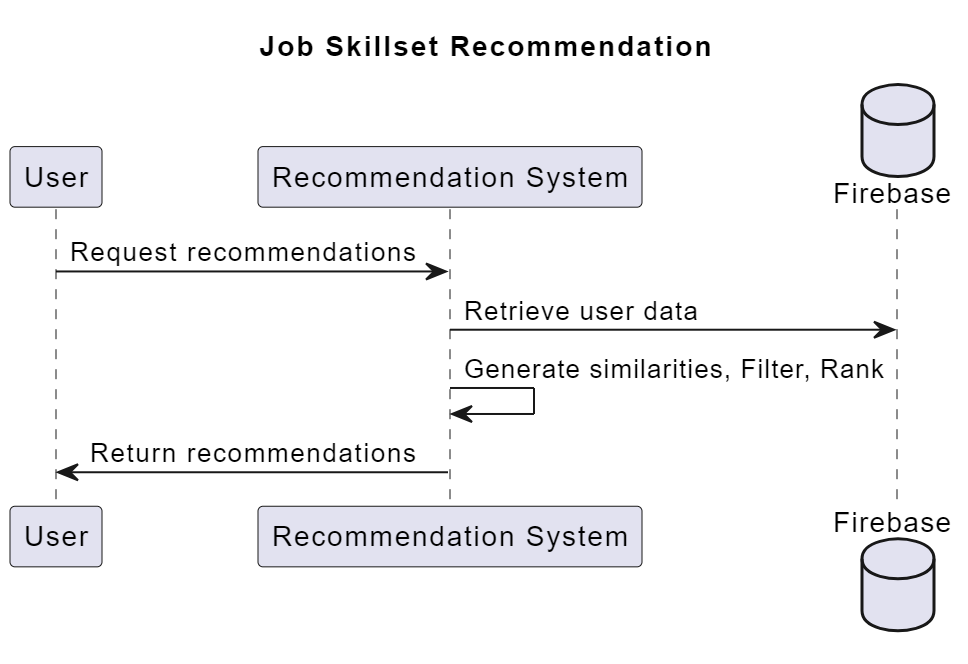
\includegraphics[width=0.8\textwidth]{3/skillset.png}
\caption{Job Skillset Recommendation Function}
\label{fig:job_skillset_recommendation}
\end{figure}

\section{Database Management}

The Database Management Module is responsible for storing and managing the dataset of courses and job skillsets. It ensures data integrity, facilitates efficient retrieval of information, and supports the updating of recommendations based on new data.\\

\begin{figure}[b]
\centering
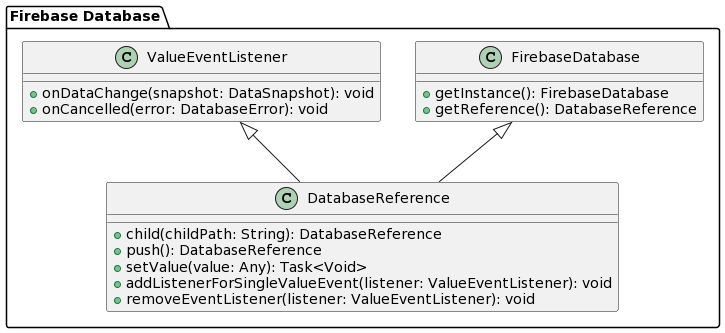
\includegraphics[width=0.8\textwidth]{3/database.png}
\caption{Database Architecture}
\label{fig:database_architecture}
\end{figure}

\section{Web Crawler}

The Web Crawler Module is responsible for gathering data from external sources to enrich the recommendation system. It automatically extracts information relevant to courses and job skillsets from websites, forums, or other online platforms. This data includes updated course listings, job postings, and industry trends.\\

\begin{figure}[t]
\centering
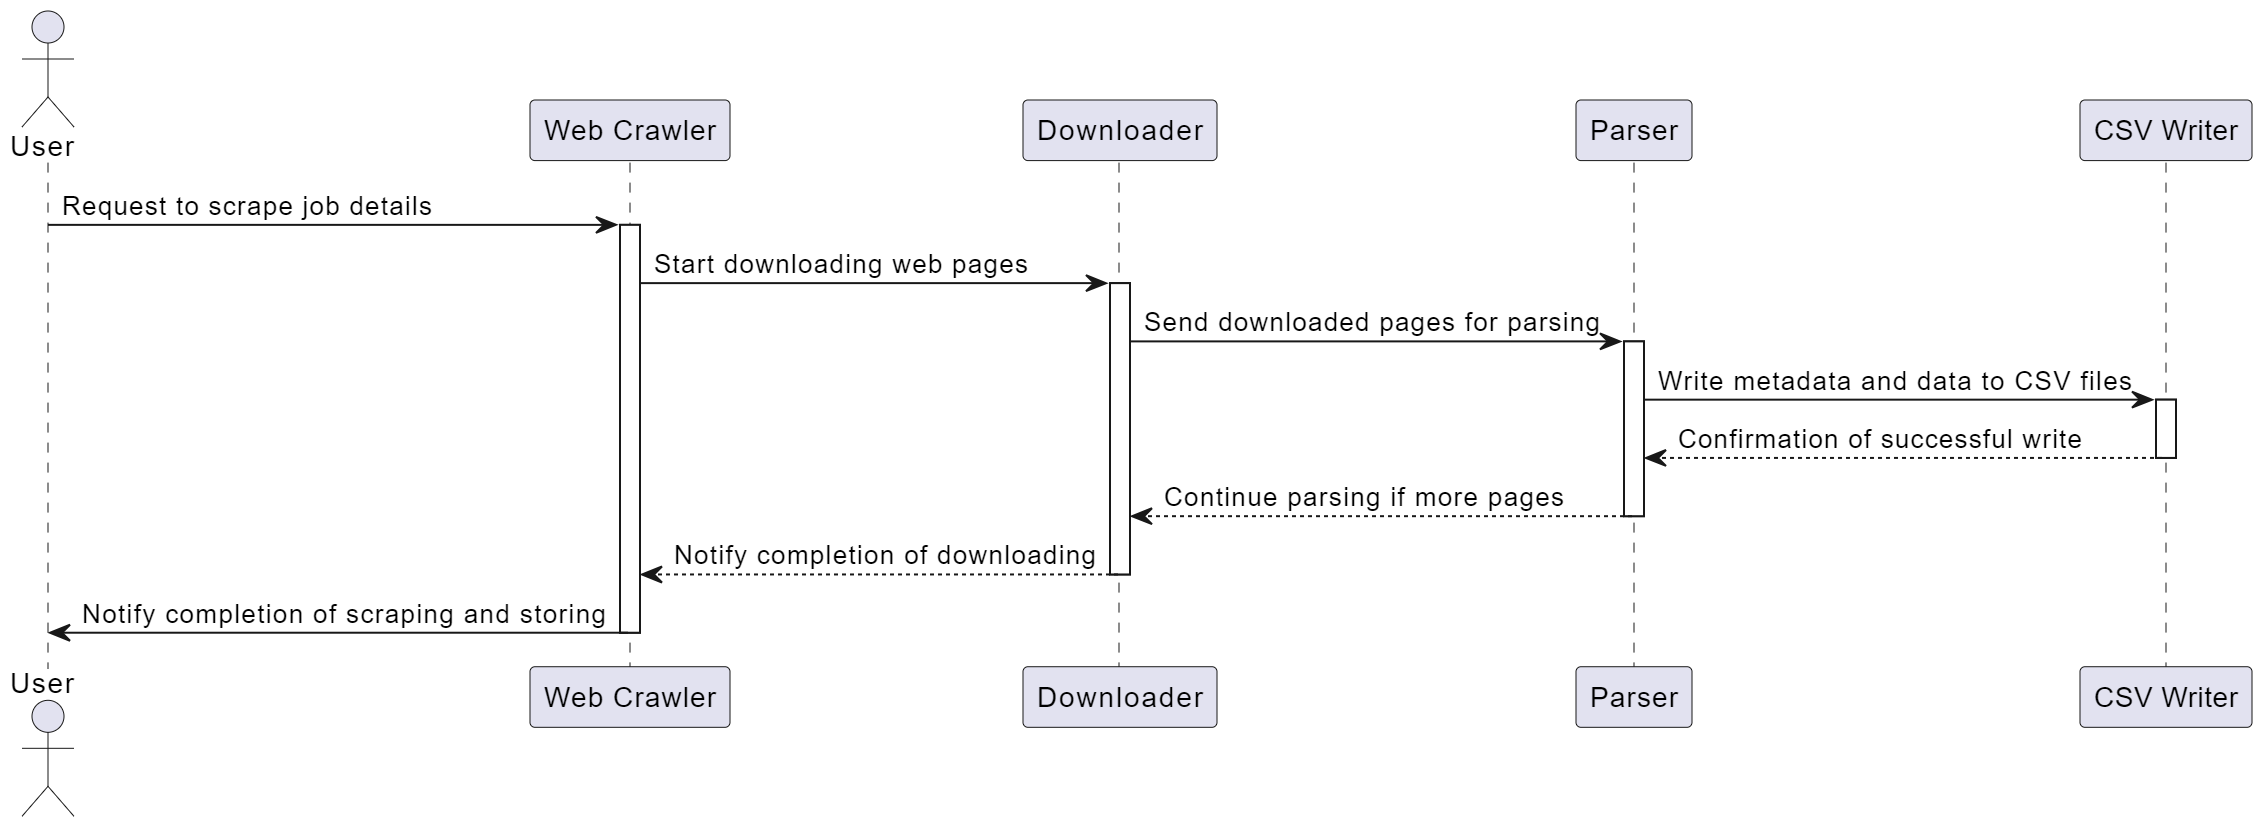
\includegraphics[width=0.8\textwidth]{3/webcrawler.png}
\caption{System Architecture for Web Crawler}
\label{fig:web_crawler}
\end{figure}
% Chapter 4

\chapter{\uppercase{Implementation of your work}} % Main chapter title
\label{chap4} % For referencing

This chapter explains about the implementation of various modules and the algorithms used in this system.

\section{Course Recommendation Generator Function}
\textbf{Workflow of the Proposed Recommendation System:}
\begin{enumerate}
    \item Retrieve course data from the course dataset and sort it by relevant attributes.
    \item Retrieve skill measurement data from the skill dataset.
    \item Retrieve user data, including preferences and career goals.
    \item Set the variable \texttt{rb} as a reference to the skill measurement data.
    \item Perform preprocessing on user input data using the \texttt{preprocessModule1} function, extracting relevant information such as user interests and career aspirations.
    \item Perform content analysis and similarity computations on the preprocessed user data using the \texttt{contentSimilarityAnalyzer} function, leveraging cosine similarity measures to identify related courses and skillsets.
    \item Iterate over each recommended item in the computed similarity data.
    \item Recommend courses and skillsets using the \texttt{recommendationGenerator} function, considering the user's preferences and career goals.
    \item Filter and refine recommendations based on availability and relevance to the user's current skill level and career trajectory.
    \item Present the recommended courses and skillsets to the user through the chatbot interface.
    \item Allow users to interact with the chatbot to provide feedback on recommendations and refine their preferences for future recommendations.
\end{enumerate}

\textbf{Algorithm for Course Recommendation Generator:}

\begin{algorithm}
\caption{Course Recommendation Generator}
\begin{algorithmic}[1]
\Require $courses$: Dataset of available courses, $skills$: Dataset of available skills, $user_preferences$: User's preferences and career goals
\Ensure $recommended_courses_and_skills$: Recommended courses and skills
\Function{RecommendationSystem}{$courses$, $skills$, $user_preferences$}
\State $content_analysis_data \gets$ Perform Content Analysis on $user_preferences$ and $skills$
\State $similarity_data \gets$ Calculate Similarity Measures on $content_analysis_data$
\State $recommended_items \gets$ Generate Recommendations from $similarity_data$ and $courses$
\State $refined_recommendations \gets$ Refine Recommendations based on $user_preferences$ and Availability
\State \Return $refined_recommendations$
\EndFunction
\end{algorithmic}
\end{algorithm}

\section{STL Decomposition Function}
\textbf{Workflow of the Proposed STL Function:}
\begin{enumerate}
    \item Input: The function takes three parameters: $data$ (the dataset), $target column$ (the column to decompose), and $period$ (the period of the seasonal component).
    \item Seasonal Decomposition: The function performs seasonal decomposition on the target column of the data using the additive model. It decomposes the time series into three components: trend, seasonal, and residual.
    \item Trend Extraction: The function extracts the trend component from the seasonal decomposition result and assigns it to the variable $trend$.
    \item Seasonal Extraction: The function extracts the seasonal component from the seasonal decomposition result and assigns it to the variable $seasonal$.
    \item Residual Extraction: The function extracts the residual component from the seasonal decomposition result and assigns it to the variable $residual$.
    \item DataFrame Construction: The function creates a new DataFrame $data\_stl$ by concatenating the original data with the trend, seasonal, and residual components. The columns of the new DataFrame are named "Trend", "Seasonal", and "Residual".
    \item DataFrame Concatenation: The function concatenates the $data$ DataFrame and the $data\_stl$ DataFrame along the columns axis.
    \item Output: The function returns the resulting $data\_stl$ DataFrame, which contains the original data along with the extracted trend, seasonal, and residual components.
\end{enumerate}

\textbf{Algorithm 4.2 Pseudocode for \texttt{stlDecomposition} Function:}
\begin{algorithm}
\caption{STL Decomposition}
\begin{algorithmic}[1]
\Require $data$: Input dataframe for the \texttt{stlDecomposition} Function, $target column$: Input string for the \texttt{stlDecomposition} Function, $period$: Input number for the \texttt{stlDecomposition} Function
\Ensure $data\_stl$: Output dataframe from \texttt{stlDecomposition} Function
\Function{STL\_DECOMPOSITION}{$data$, $target column$, $period$}
    \State $result \gets$ seasonal decompose($data$[$target column$], model='additive', period=$period$)
    \State $trend \gets result.trend$
    \State $seasonal \gets result.seasonal$
    \State $residual \gets result.resid$
    \State $data\_stl \gets$ pd.concat([$trend$, $seasonal$, $residual$], axis=1)
    \State $data\_stl$.columns $\gets$ ["Trend", "Seasonal", "Residual"]
    \State $data\_stl \gets$ pd.concat([$data$, $data\_stl$], axis=1)
    \State \Return $data\_stl$
\EndFunction
\end{algorithmic}
\end{algorithm}


\section{Perform Imputation Function}

\textbf{Workflow of the Proposed Imputation Function:}
\begin{enumerate}
    \item Input: The function takes a single parameter $X$, which is the input dataset containing missing values.
    \item Imputer Initialization: The function initializes an instance of the IterativeImputer class as $imputer$. The IterativeImputer is a class for imputing missing values by modeling each feature with missing values as a function of other features.
    \item Imputation: The function uses the fit transform method of the imputer object to perform imputation on the input dataset $X$. This method fits the imputer model on $X$ and transforms $X$ by filling in the missing values. The result is stored in $X\_filled$.
    \item DataFrame Construction: The function creates a new DataFrame $X\_imputed$ using the filled data $X\_filled$. The columns of the new DataFrame are set to be the same as the columns of the original $X$ dataset.
    \item Output: The function returns the resulting $X\_imputed$ DataFrame, which contains the input dataset $X$ with the missing values imputed.
\end{enumerate}

\textbf{Algorithm 4.3 Pseudocode for \texttt{performImputation} Function:}
\begin{algorithm}
\caption{Perform Imputation}
\begin{algorithmic}[1]
\Require $X$: Input dataframe for the \texttt{performImputation} Function
\Ensure $X\_imputed$: Output dataframe from \texttt{performImputation} Function
\Function{PERFORM\_IMPUTATION}{$X$}
    \State $imputer \gets$ IterativeImputer(estimator=HistGradientBoostingRegressor())
    \State $X\_filled \gets$ imputer.fit transform($X$)
    \State $X\_imputed \gets$ pd.DataFrame($X\_filled$, columns = $X$.columns)
    \State \Return $X\_imputed$
\EndFunction
\end{algorithmic}
\end{algorithm}

\section{Random Forest Regressor Algorithm}

\textbf{Workflow of the Proposed Model:}
\begin{enumerate}
    \item Initialize an empty random forest model.
    \item Repeat the following steps for each tree in the forest (100 trees in total):
    \begin{enumerate}
        \item Sample a bootstrap dataset from the training data. This involves randomly selecting samples from the training dataset with replacement, creating a new dataset of the same size as the original but with some duplicate samples.
        \item Create a decision tree with a maximum depth of 5. The decision tree will recursively split the dataset based on the features and their values, aiming to minimize the mean squared error of the predicted values.
        \item Fit the decision tree to the bootstrap dataset. The decision tree algorithm will determine the optimal splitting points for each node based on the selected features and their values.
        \item Add the decision tree to the random forest model.
    \end{enumerate}
    \item Once all the trees are added to the forest, the model is ready for prediction.
    \item To make a prediction, provide an input feature vector to the random forest model.
    \item Each tree in the forest independently predicts the output value based on the input feature vector.
    \item The final prediction is obtained by aggregating the predictions of all the trees. In the case of regression, this is commonly done by taking the average of the individual tree predictions.
    \item The trained random forest model can be used to make predictions on new unseen data by passing the feature vectors through each tree in the forest and aggregating the results.
\end{enumerate}

\textbf{Algorithm 4.4 Pseudocode for Random Forest Regressor:}
\begin{algorithm}
\caption{Random Forest Regressor}
\begin{algorithmic}[1]
\Require $X$: Input features, $Y$: Output labels, $n\_estimators$: Number of trees in the random forest, $max\_depth$: Maximum depth of each tree
\Ensure $forest$: Trained random forest model
\Function{RANDOM\_FOREST\_REGRESSOR}{$X$, $Y$, $n\_estimators$, $max\_depth$}
    \State Initialize an empty list $forest$
    \For{$i$ in range($n\_estimators$)}
        \State Sample a bootstrap dataset $X\_sample$, $Y\_sample$ from $X$, $Y$
        \State Create a decision tree $T_i$ with maximum depth $max\_depth$
        \State Fit the decision tree $T_i$ to $X\_sample$, $Y\_sample$
        \State Add $T_i$ to the forest $forest$
    \EndFor
    \State \Return $forest$
\EndFunction
\end{algorithmic}
\end{algorithm}

\section{Gradient Boosting Regressor Algorithm}

\textbf{Workflow of the Proposed Model:}
\begin{enumerate}
    \item Initialize the boosting model by setting the initial prediction value for each sample in the training data.
    \item Repeat the following steps for each boosting stage (100 stages in total):
    \begin{enumerate}
        \item Compute the negative gradient of the loss function with respect to the current predictions. This represents the ”residuals” or errors that the model needs to correct.
        \item Fit a regression tree to the negative gradients. The tree is trained to predict the negative gradients, which captures the information to correct the previous predictions.
        \item Determine the step size (learning rate) by minimizing the loss function. The step size controls the contribution of each tree to the final prediction and helps prevent overfitting.
        \item Update the model by adding the current tree’s predictions, scaled by the step size, to the previous predictions. This update corrects the previous predictions based on the new information learned from the current tree.
    \end{enumerate}
    \item Once all the boosting stages are completed, the model is ready for prediction.
    \item To make a prediction, provide an input feature vector to the gradient boosting model.
    \item Each regression tree in the ensemble independently predicts the output value based on the input feature vector.
    \item The final prediction is obtained by summing the predictions of all the regression trees, weighted by the learning rate.
    \item The trained gradient boosting model can be used to make predictions on new unseen data by passing the feature vectors through each tree in the ensemble and aggregating the results.
\end{enumerate}

\textbf{Algorithm 4.5 Pseudocode for Gradient Boosting Regressor:}
\begin{algorithm}
\caption{Gradient Boosting Regressor}
\begin{algorithmic}[1]
\Require $X$: Input features, $Y$: Output labels, $n\_estimators$: Number of boosting stages to perform, $max\_depth$: Maximum depth of each tree, $min\_samples\_leaf$: Minimum number of samples required to be at a leaf node, $learning\_rate$: Learning rate shrinks the contribution of each tree
\Ensure $F_m(X)$: Trained gradient boosting model
\Function{GRADIENT\_BOOSTING\_REGRESSOR}{$X$, $Y$, $n\_estimators$, $max\_depth$, $min\_samples\_leaf$, $learning\_rate$}
    \State Initialize $F_0$ as a constant value
    \For{$m$ in range($n\_estimators$)}
        \State Compute the negative gradient $r_{im}$ for each sample $i$ using the loss function
        \State Train a regression tree $h_m(X)$ to the negative gradients
        \State Compute the step size $\gamma_m$ by minimizing the loss function
        \State Update the function $F_m(X) = F_{m-1}(X) + \gamma_m \cdot h_m(X)$
    \EndFor
    \State \Return $F_m(X)$
\EndFunction
\end{algorithmic}
\end{algorithm}

\section{Histogram Gradient Boosting Regressor Algorithm}

\textbf{Workflow of the Proposed Model:}
\begin{enumerate}
    \item Initialize the histogram-based gradient boosting model.
    \item Repeat the following steps for each boosting stage (100 stages in total):
    \begin{enumerate}
        \item Compute the negative gradients (residuals) of the loss function with respect to the current predictions.
        \item Construct histograms for each feature in the training data, partitioning the feature space into discrete bins.
        \item For each feature, find the optimal splits to minimize the loss function within each bin, considering the negative gradients.
        \item Build a tree structure using the best splits for each feature, where the nodes represent the bins and the leaves represent the predictions.
        \item Update the model by adding the predictions of the current tree to the previous predictions, weighted by the learning rate.
    \end{enumerate}
    \item Once all the boosting stages are completed, the model is ready for prediction.
    \item To make a prediction, provide an input feature vector to the histogram-based gradient boosting model.
    \item The feature values are binned based on the histograms created during training, and the model navigates the tree structure to find the corresponding prediction.
    \item The final prediction is obtained by summing the predictions of all the trees, weighted by the learning rate.
    \item The trained histogram-based gradient boosting model can be used to make predictions on new unseen data by following the same binning and tree traversal process as during training.
\end{enumerate}

\textbf{Algorithm 4.6 Pseudocode for Histogram Gradient Boosting Regressor:}
\begin{algorithm}
\caption{Histogram Gradient Boosting Regressor}
\begin{algorithmic}[1]
\Require $X$: Input features, $Y$: Output labels, $max\_iter$: Maximum number of iterations (boosting stages) to perform, $max\_depth$: Maximum depth of each tree, $min\_samples\_leaf$: Minimum number of samples required to be at a leaf node
\Ensure $F_m(X)$: Trained histogram-based gradient boosting model
\Function{HIST\_GRADIENT\_BOOSTING\_REGRESSOR}{$X$, $Y$, $max\_iter$, $max\_depth$, $min\_samples\_leaf$}
    \State Initialize $F_0$ as a constant value
    \For{$m$ in range($max\_iter$)}
        \State Compute the negative gradient $r_{im}$ for each sample $i$ using the loss function
        \State Train a histogram-based gradient boosting tree $T_m(X)$ to the negative gradients
        \State Compute the step size $\gamma_m$ by minimizing the loss function
        \State Update the function $F_m(X) = F_{m-1}(X) + \gamma_m \cdot T_m(X)$
    \EndFor
    \State \Return $F_m(X)$
\EndFunction
\end{algorithmic}
\end{algorithm}
% Chapter 5

\chapter{\uppercase{Results and Performance Analysis}} % Main chapter title
\label{chap5}
The complexity analysis provides insights into the efficiency of the algorithms used in our recommendation system in terms of time and space requirements.

\section{Time Complexity}

The time complexity of the recommendation algorithms utilized in our project can be approximated as $O(n \log n)$, where $n$ is the number of available items (courses or job skillsets). The primary factor contributing to this complexity is the sorting operation performed on the available items to determine the most relevant recommendations. The sorting operation typically has an average time complexity of $O(n \log n)$ when using efficient sorting algorithms. Thus, as the number of available items increases, the time required to generate recommendations scales logarithmically.

\section{Space Complexity}

In terms of space complexity, the recommendation algorithms utilized in our project have a space complexity of $O(1)$. The space requirements remain constant irrespective of the input size, as the algorithms mainly utilize additional space for storing variables and data structures. This efficient space utilization ensures that the memory consumption does not grow with the size of the available items, making the algorithms efficient in terms of space usage.

\section{Evaluation of Recommendation System}

The recommendation system used in this project demonstrates efficiency, adaptability, accuracy, scalability, and optimal resource usage. By intelligently recommending courses and job skillsets based on factors such as user preferences and similarity measures, the system ensures an optimized learning and career development experience for users. Its adaptability allows for customization to specific user contexts, while its accuracy matches recommendations to users' interests and career goals. With a time complexity of $O(n \log n)$ and a space complexity of $O(1)$, the recommendation system handles a large number of items efficiently and utilizes memory resources optimally. Overall, the recommendation system offers a robust solution for personalized course and job skillset recommendations, enhancing the learning and career development journey for users.

\chapter{\uppercase{Conclusion and Future Work}}
\label{chap:conclusion}
\section{\uppercase{Conclusion}}
In conclusion, the development and implementation of the recommendation system integrated into a chatbot application represent a significant step towards addressing the challenges individuals face in navigating the rapidly evolving job market. By leveraging item-based recommendation techniques, particularly cosine similarity measures, the system effectively assists users in identifying relevant courses and acquiring the necessary skills to meet the demands of various industries.

The recommendation system analyzes a vast dataset of courses and job requirements, employing similarity measures to identify relevant courses and skillsets that closely align with a user's interests and career goals. The integration of the recommendation system into a chatbot application further enhances user experience by providing a conversational interface for interaction, allowing users to receive personalized recommendations and explore career development opportunities in a seamless and intuitive manner.

Overall, the recommendation system serves as a valuable tool for individuals seeking to enhance their skillsets and advance their careers in an increasingly competitive job market. By facilitating access to relevant learning resources and maximizing users' potential for professional growth and success, the system contributes to the ongoing efforts to bridge the skills gap and promote lifelong learning in the digital age.
\\ \\ \\

\section{\uppercase{Future Work}}

Moving forward, there are several avenues for enhancing the recommendation system's efficacy and user experience. Firstly, continuous refinement of the recommendation algorithms is paramount. Incorporating advanced machine learning techniques, such as deep learning models, and fine-tuning parameters based on user feedback can improve the accuracy and relevance of course suggestions. Moreover, exploring novel approaches like collaborative filtering and hybrid recommendation systems could provide additional insights into users' preferences and needs.

Expanding the dataset used for analysis represents another critical area for future development. Integrating data from diverse sources, including job market trends, emerging technologies, and user behavior patterns, can enrich the recommendation system's knowledge base. This broader dataset can offer users a more comprehensive range of course options tailored to their career aspirations and industry demands.

Additionally, enhancing the conversational capabilities of the chatbot interface is essential to foster greater user engagement and satisfaction. Leveraging advancements in natural language processing (NLP) and sentiment analysis can enable the chatbot to understand user queries more effectively and provide more contextually relevant responses. Furthermore, incorporating interactive features such as voice recognition and personalized chat experiences can further elevate the user experience and encourage continued interaction with the system.

% Start a new page
\cleardoublepage
% Create a phantom section
\phantomsection

% \bibliographystyle{auapalike}
\bibliographystyle{unsrt}
\nocite{*} % This command includes all references even if they are not cited. You might want to remove it once references are cited in your document.
\phantomsection

% Add the references section to the table of contents
\addcontentsline{toc}{chapter}{REFERENCES}
\begin{spacing}{1} % Adjust spacing in the bibliography
\bibliography{publication} % Include the bibliography file named "publication.bib"
\end{spacing}

% Start a new page
\newpage
\clearpage

% Add new pages to the table of contents, list of tables, and list of figures
\addtocontents{toc}{\protect\newpage}
\addtocontents{lot}{\protect\newpage}
\addtocontents{lof}{\protect\newpage}

% End of the document
\end{document} 